\documentclass{article}
\usepackage[utf8]{inputenc}
\usepackage{authblk}
\usepackage[margin=1.7in]{geometry}
\usepackage{wrapfig}
\usepackage{graphicx}

\title{Data Aggregation \& Analysis System for Intelligent Agriculture: Design Document}
\author[1]{Panagiotis Stanitsas \thanks{stani078@umn.edu}}
\author[1]{Jacob Quant \thanks{quant006@umn.edu}}
\author[1]{Nabil Cheikh  \thanks{cheik004@d.umn.edu}}

	
\affil[1]{Department of Computer Science and Engineering, University of Minnesota, Minneapolis, MN 55455 USA}

\renewcommand\Authands{ and }
\date{}

\begin{document}

\maketitle

\begin{abstract}
\end{abstract}

\section{Motivation}
Over the past decade a great amount of attention has been received in the area of intelligent system development in precision agriculture. Methods along the lines of satellite and drone image processing as well as technologically advanced sensing techniques are deployed in an effort to increase the efficiency of modern crops while optimizing the quantities of the necessary resources (e.g. fertilizers, water). Figure \ref{fig:HighLev} 

\begin{wrapfigure}{l}{3in}
\begin{center}
   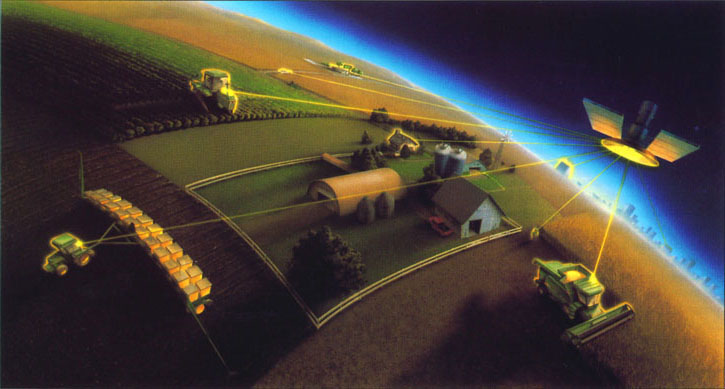
\includegraphics[width=1\linewidth,trim={0 0 0 0cm},clip]{Images/HighLevel.jpg}
\end{center}
\vspace{-0.2in}
   \caption{\footnotesize{A High-Level Overview of Precision Agriculture.}}
   \label{fig:HighLev}
   %\vspace{-0.08in}
\end{wrapfigure}

\noindent illustrates a high-level view of the the multistage structure of modern Precision Agriculture according to which information is aggregated at a central hub, then processed and based on the results, all agents receive a plan of action regarding irrigation, fertilization, harvesting and planting.  Capitalizing on the continuous effort of reducing the associated cost with Precision Agriculture applications, cheap sensing solutions can be implemented in order to provide valuable information even on the farmer's smart phones. In particular, the scenario that this project aims to replicate is the delivery of information, which is harvested in the field, to a mobile device based on user defined queries. 
\begin{wrapfigure}{r}{2in}
\begin{center}
   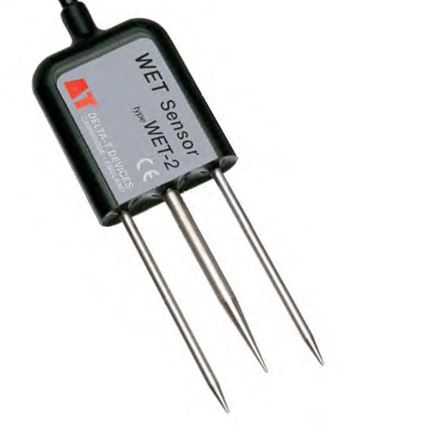
\includegraphics[width=1\linewidth,trim={0 0 0 0cm},clip]{Images/HumSens.jpg}
\end{center}
\vspace{-0.2in}
   \caption{\footnotesize{Soil Humidity Sensor.}}
   \label{fig:Humsens}
   %\vspace{-0.08in}
\end{wrapfigure}

Sensors that can measure the humidity of the soil can be purchased at a very low price (\$10 - \$20), while constructing a wireless network (e.g. ZigBee modules) that is capable of carrying the sensor measurements to a central processing location can be also completed within a constricted budget. Figure \ref{fig:Humsens} presents a soil humidity sensor distributed by Hoskin Scientific and has the ability to measures water content and temperature directly within the root zone. Rather than using sophisticated devices to deliver informtatio this effort promotes the use of the user In that way, utilizing low-cost sensor measurements, farmers can monitor the humidity (of the soil) and plan accordingly for their irrigation strategies.







\section{Problem Statement}

\section{Relevant work}



\section{Front-end Implementation}

\section{Data Analytics}

\section{Back-end Implementation}

\section{Module Aggregation}



\end{document}
